\begin{tabular}{lc|cc}
\hline
& Pattern & $\rho$ & p-value \\\hline
%%%%%%%%%%%%%%%%%%%%%%%%%%%%%%%%%%%%%%%%%%%%%%%%%%%%
\rb{\emph{3-node}} &
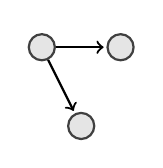
\begin{tikzpicture}[shorten >=1pt,->,scale=0.5]  
        \tikzstyle{sentence}=[circle,thick,draw=black!75,fill=black!10,minimum size=2mm]
        \tikzstyle{edge}=[draw, thick]
       \begin{scope}
         \node [sentence] (s1) at (0,2) {\tiny{}};
         \node [sentence] (s2) at (2,2) {\tiny{}};
         \node [sentence] (s3) at (1,0) {\tiny{}}; 
         \path[edge] (s1) edge [above] node[font=\tiny] {} (s2);
         \path[edge] (s1) edge [above] node[font=\tiny] {} (s3);
        \end{scope}        
\end{tikzpicture}
      &	\rb{0.43} & \rb{0.024}
      \\\hline
\rb{\emph{4-node}} &
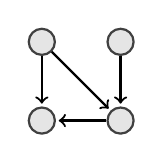
\begin{tikzpicture}[shorten >=1pt,->,scale=0.5]  
        \tikzstyle{sentence}=[circle,thick,draw=black!75,fill=black!10,minimum size=1mm]
        \tikzstyle{edge}=[draw, thick]
       \begin{scope}
         \node [sentence] (s1) at (0,2) {\tiny{}};
         \node [sentence] (s2) at (2,2) {\tiny{}};
         \node [sentence] (s3) at (2,0) {\tiny{}};
         \node [sentence] (s4) at (0,0) {\tiny{}};  
         \path[edge] (s1) edge [above] node[font=\tiny] {} (s3);
         \path[edge] (s1) edge [above] node[font=\tiny] {} (s4);
         \path[edge] (s2) edge [above] node[font=\tiny] {} (s3);
         \path[edge] (s3) edge [above] node[font=\tiny] {} (s4);
        \end{scope}        
      \end{tikzpicture}
      &	\rb{-0.45} & \rb{0.018}
      
       \\
&
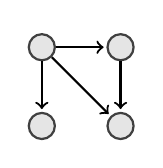
\begin{tikzpicture}[shorten >=1pt,->,scale=0.5]  
        \tikzstyle{sentence}=[circle,thick,draw=black!75,fill=black!10,minimum size=1mm]
        \tikzstyle{edge}=[draw, thick]
       \begin{scope}
         \node [sentence] (s1) at (0,2) {\tiny{}};
         \node [sentence] (s2) at (2,2) {\tiny{}};
         \node [sentence] (s3) at (2,0) {\tiny{}};
         \node [sentence] (s4) at (0,0) {\tiny{}};  
         \path[edge] (s1) edge [above] node[font=\tiny] {} (s2);
         \path[edge] (s1) edge [above] node[font=\tiny] {} (s3);
         \path[edge] (s1) edge [above] node[font=\tiny] {} (s4);
         \path[edge] (s2) edge [above] node[font=\tiny] {} (s3);
        \end{scope}        
      \end{tikzpicture}
      &	\rb{+0.39} & \rb{0.047}
      \\
&
      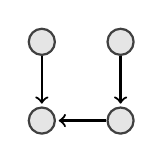
\begin{tikzpicture}[shorten >=1pt,->,scale=0.5]  
        \tikzstyle{sentence}=[circle,thick,draw=black!75,fill=black!10,minimum size=1mm]
        \tikzstyle{edge}=[draw, thick]
       \begin{scope}
         \node [sentence] (s1) at (0,2) {\tiny{}};
         \node [sentence] (s2) at (2,2) {\tiny{}};
         \node [sentence] (s3) at (2,0) {\tiny{}};
         \node [sentence] (s4) at (0,0) {\tiny{}};  
         \path[edge] (s1) edge [above] node[font=\tiny] {} (s4);
         \path[edge] (s2) edge [above] node[font=\tiny] {} (s3);
         \path[edge] (s3) edge [above] node[font=\tiny] {} (s4);
        \end{scope}        
      \end{tikzpicture}
      &	 \rb{-0.43}  & \rb{0.024}
      \\
&
      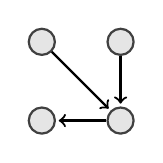
\begin{tikzpicture}[shorten >=1pt,->,scale=0.5]  
        \tikzstyle{sentence}=[circle,thick,draw=black!75,fill=black!10,minimum size=1mm]
        \tikzstyle{edge}=[draw, thick]
       \begin{scope}
         \node [sentence] (s1) at (0,2) {\tiny{}};
         \node [sentence] (s2) at (2,2) {\tiny{}};
         \node [sentence] (s3) at (2,0) {\tiny{}};
         \node [sentence] (s4) at (0,0) {\tiny{}};  
         \path[edge] (s1) edge [above] node[font=\tiny] {} (s3);
         \path[edge] (s2) edge [above] node[font=\tiny] {} (s3);
         \path[edge] (s3) edge [above] node[font=\tiny] {} (s4);
        \end{scope}        
      \end{tikzpicture}
      &	\rb{-0.59} & \rb{0.001}
      \\
&
      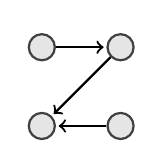
\begin{tikzpicture}[shorten >=1pt,->,scale=0.5]  
        \tikzstyle{sentence}=[circle,thick,draw=black!75,fill=black!10,minimum size=1mm]
        \tikzstyle{edge}=[draw, thick]
       \begin{scope}
         \node [sentence] (s1) at (0,2) {\tiny{}};
         \node [sentence] (s2) at (2,2) {\tiny{}};
         \node [sentence] (s3) at (2,0) {\tiny{}};
         \node [sentence] (s4) at (0,0) {\tiny{}};  
         \path[edge] (s1) edge [above] node[font=\tiny] {} (s2);
         \path[edge] (s2) edge [above] node[font=\tiny] {} (s4);
         \path[edge] (s3) edge [above] node[font=\tiny] {} (s4);
        \end{scope}        
      \end{tikzpicture}
      &	\rb{-0.55} & \rb{0.003}
      \\
&
      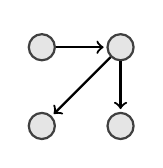
\begin{tikzpicture}[shorten >=1pt,->,scale=0.5]  
        \tikzstyle{sentence}=[circle,thick,draw=black!75,fill=black!10,minimum size=1mm]
        \tikzstyle{edge}=[draw, thick]
       \begin{scope}
         \node [sentence] (s1) at (0,2) {\tiny{}};
         \node [sentence] (s2) at (2,2) {\tiny{}};
         \node [sentence] (s3) at (2,0) {\tiny{}};
         \node [sentence] (s4) at (0,0) {\tiny{}};  
         \path[edge] (s1) edge [above] node[font=\tiny] {} (s2);
         \path[edge] (s2) edge [above] node[font=\tiny] {} (s3);
         \path[edge] (s2) edge [above] node[font=\tiny] {} (s4);
        \end{scope}        
      \end{tikzpicture}
      &	\rb{-0.55} & \rb{0.003}
      
\end{tabular}

